% --- Conteúdo ATUALIZADO para Tabela&Grafico/selection_sort.tex ---

\qquad A seguir são apresentados os resultados obtidos na execução do algoritmo \textit{Selection Sort}.

% --- IMAGEM DA TABELA DO SELECTION SORT ---
\begin{figure}[h!]
    \centering
    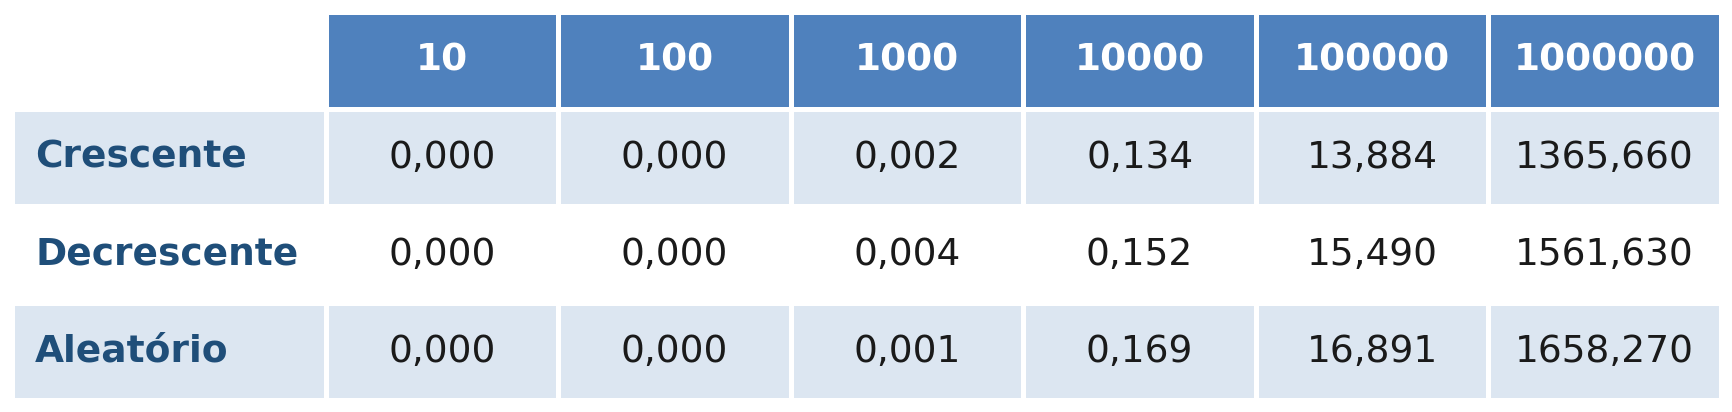
\includegraphics[width=1.0\textwidth]{Imagens/Selection Sort/tabela_selection.png}
    \caption{Tabela de tempo de execução (em segundos) do \textit{Selection Sort} (elaborado pelo autor).}
    \label{fig:tabela_selection}
\end{figure}

% --- IMAGEM DO GRÁFICO DO SELECTION SORT ---
\begin{figure}[h!]
    \centering
    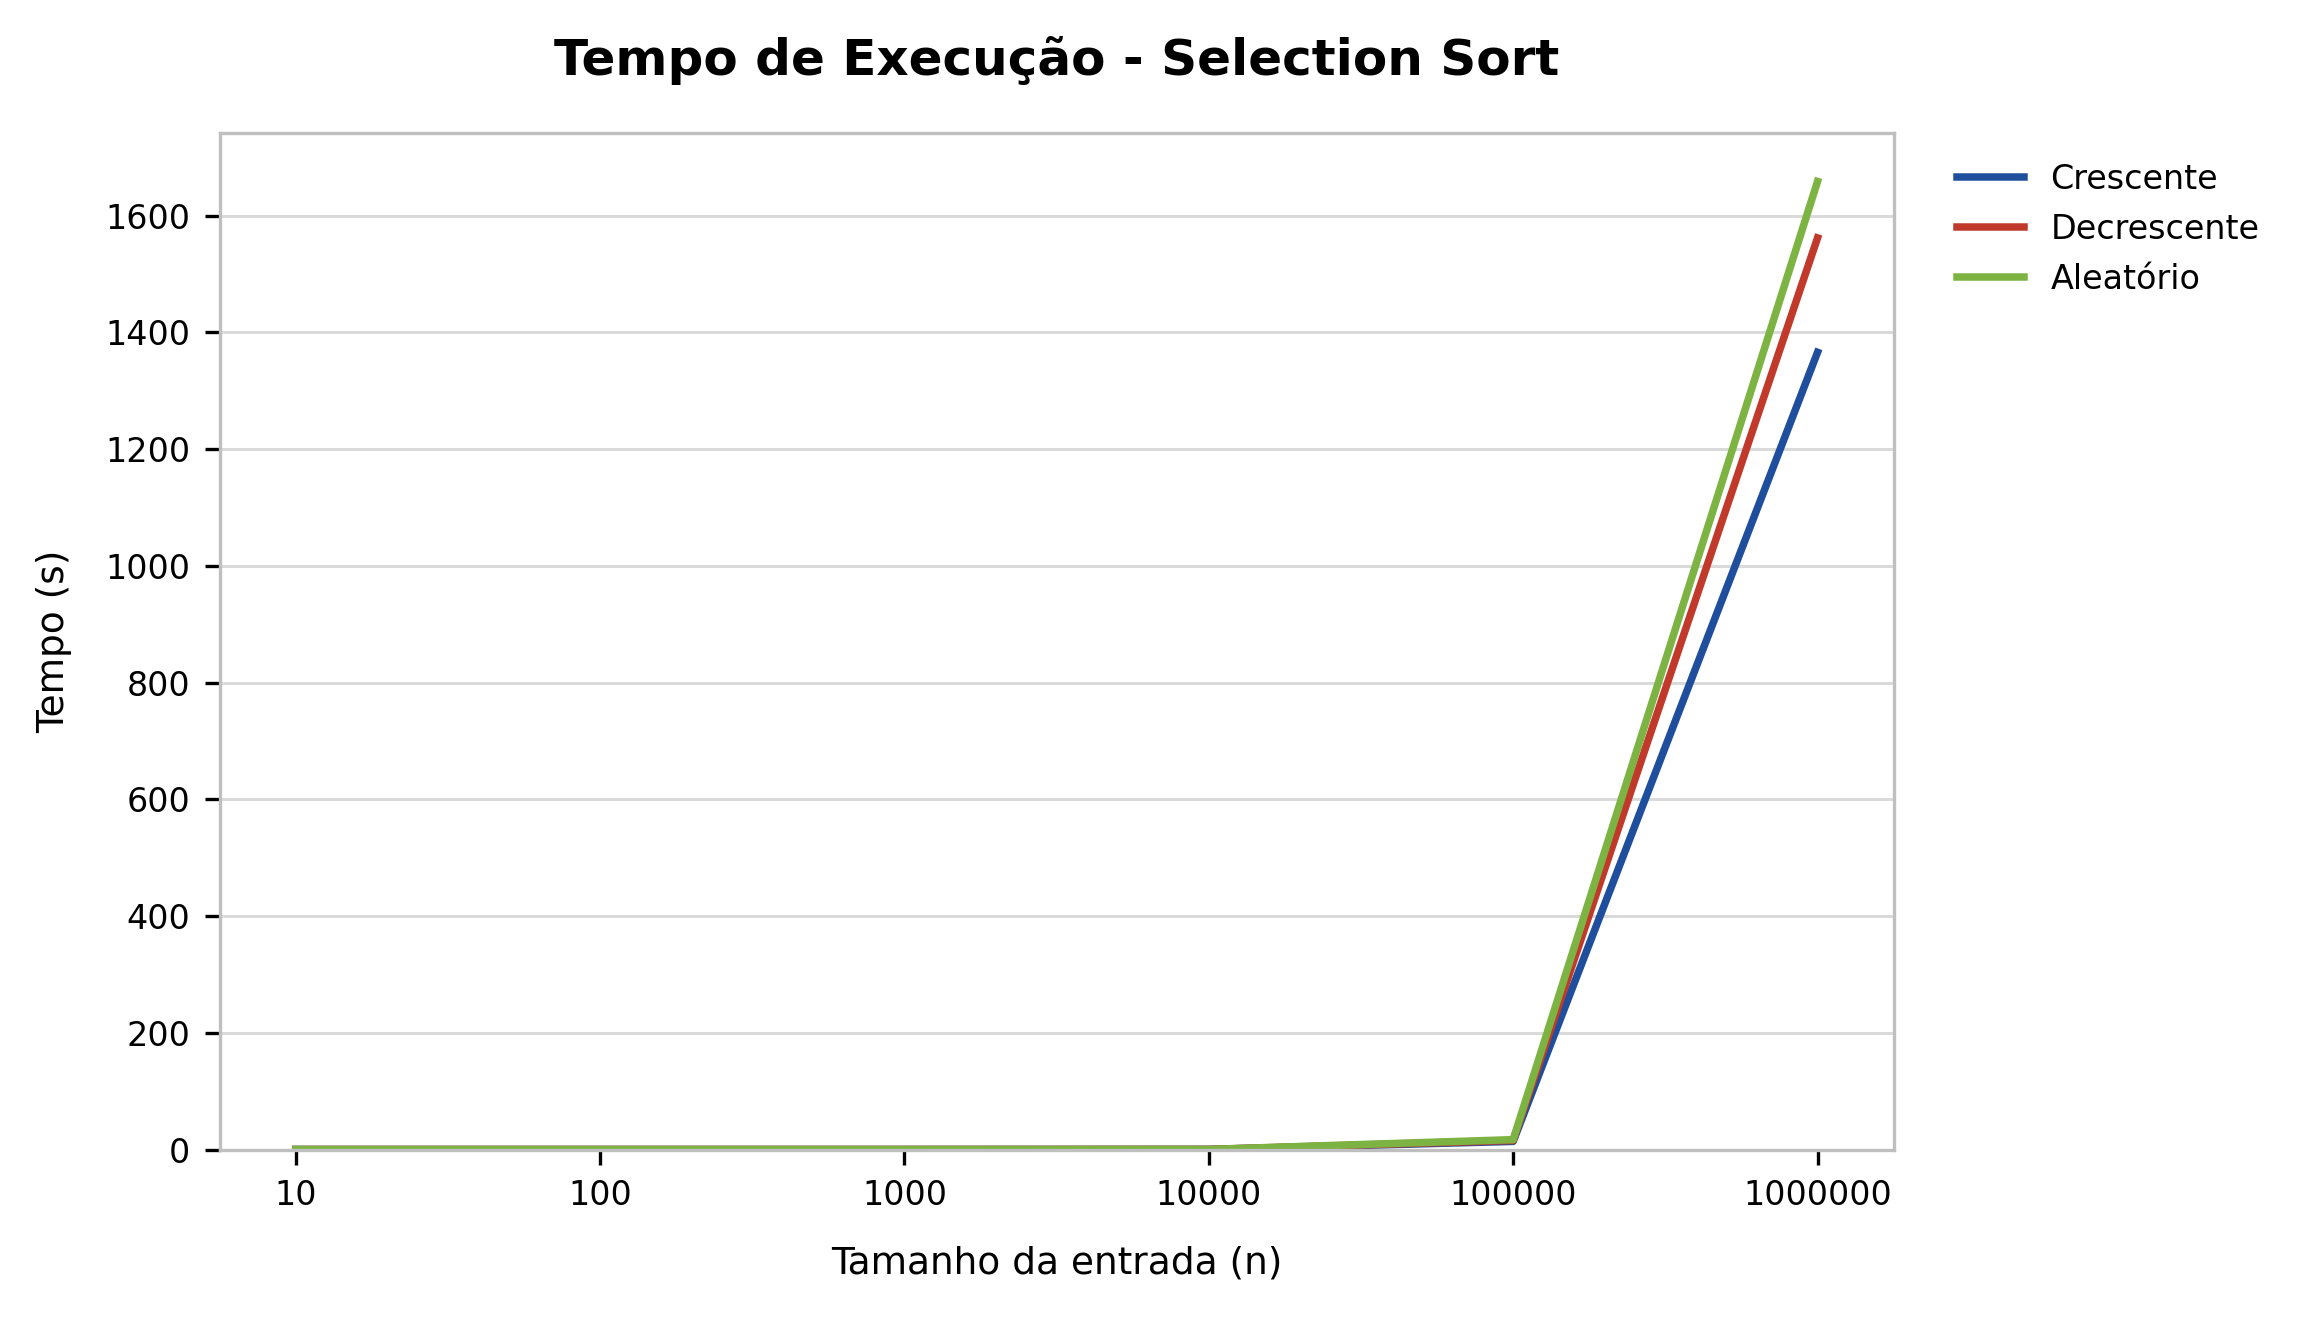
\includegraphics[width=1.0\textwidth]{Imagens/Selection Sort/grafico_selection.png}
    \caption{Desempenho do Algoritmo \textit{Selection Sort} (elaborado pelo autor).}
    \label{fig:grafico_selection}
\end{figure}

% --- ANÁLISE DOS RESULTADOS DO SELECTION SORT ---

\qquad Os dados da Figura \ref{fig:tabela_selection} e o gráfico da Figura \ref{fig:grafico_selection} evidenciam a principal característica do \textit{Selection Sort}: a pouca sensibilidade à ordem inicial dos dados. Para as entradas de 10 e 100 elementos, os tempos registrados foram de 0,000 segundo em todos os cenários, o que indica apenas que a duração ficou abaixo da precisão do relógio utilizado.

\begin{itemize}
    \item \textbf{Desempenho consistente entre os cenários:} os tempos para um milhão de elementos foram de 1.365,660 segundos (crescente), 1.561,630 segundos (decrescente) e 1.658,270 segundos (aleatório), todos entre 22 e 28 minutos. A diferença entre o menor e o maior tempo é de aproximadamente 21\%, valor pequeno quando comparado à diferença de mais de 160\% observada no \textit{Bubble Sort} entre o melhor e o pior cenário.

    \item \textbf{Origem dessa estabilidade:} o algoritmo executa sempre o mesmo número de comparações, $\frac{n(n-1)}{2}$, independentemente da ordem inicial do vetor, pois o laço interno precisa percorrer toda a porção não ordenada para localizar o menor elemento. O número de trocas também é fixo em $n-1$. A pequena variação observada entre os cenários vem apenas das atualizações do índice \texttt{min\_idx}, que ocorrem com frequências diferentes conforme a distribuição dos dados.

    \item \textbf{Complexidade quadrática:} o crescimento dos tempos acompanha o esperado para $O(n^2)$. Ao passar de 100.000 para 1.000.000 de elementos, entrada dez vezes maior, o tempo do caso aleatório passou de 16,891 s para 1.658,270 s, um aumento de aproximadamente 98 vezes, valor bastante próximo das 100 vezes previstas pela análise teórica.
\end{itemize}

\qquad Comparado ao \textit{Bubble Sort}, o \textit{Selection Sort} apresentou desempenho superior em todos os cenários com um milhão de elementos, especialmente nas entradas decrescente e aleatória, onde foi cerca de 2,4 vezes mais rápido. Essa vantagem decorre do menor número de trocas realizadas: enquanto o \textit{Bubble Sort} pode efetuar uma troca a cada comparação, o \textit{Selection Sort} realiza no máximo $n-1$ trocas ao todo.

\qquad De modo geral, os testes mostram um algoritmo de desempenho estável e previsível, mas ainda assim inadequado para entradas grandes, já que não obtém qualquer vantagem quando os dados estão parcialmente ordenados.

\FloatBarrier